\documentclass[13pt,a4paper]{report}
\usepackage[utf8]{inputenc}
\usepackage{enumerate}
\usepackage{tikz}
\usepackage{pgfplots}
\usetikzlibrary{plotmarks}
\usepackage{amssymb}
\usepackage{xcolor}

\usepackage{verbatim}
%\usepackage{enumitem}
\usepackage{listings}

\renewcommand{\thesection}{\arabic{section}}
\renewcommand\theparagraph{\thesubsubsubsection.\arabic{paragraph}} % optional; useful if paragraphs are to be numbered


\begin{document}
	
\begin{titlepage}
	\centering
	\vspace{2cm}
	{\huge\bfseries Report of Project of Semester S1: Nonparametric method for image analysis \par}
	\vspace{2cm}
	{\Large\itshape Students:\\
		Loc Thi Thuy Linh\\
		Nguyen Duc Tho\par}
	\vfill
	supervised by\par
	\large Nghiem Thi Phuong \& Tran Giang Son\\
	ICT Department, USTH\par
	\vfill
% Bottom of the page
	{\large \today\par}
\end{titlepage}

\tableofcontents{}
\newpage

\section{Introduction}

\subsection{What is clustering?}

\subsection{Why is clustering used?}

\subsection{How does clustering work?}

\subsection{Clustering categories}
\begin{enumerate}[a.]
	\item Parametric
	\item Non-parametric
\end{enumerate}

\section{K-means}

\subsection{What?}

\subsection{Why?}

\subsection{How?}

\subsection{Advantages and disadvantages}
%lead to the next part


\section{Non-parametric: Meanshift}

\subsection{What?}
Mean shift is a non-parametric feature-space analysis technique for locating the maxima of a density function, a so-called mode-seeking algorithm\textsuperscript{2.1}
\pgfplotsset{grid style={dashed,gray}}
\pgfplotsset{minor grid style={dashed,red}}
\pgfplotsset{major grid style={dotted,green!50!black}}


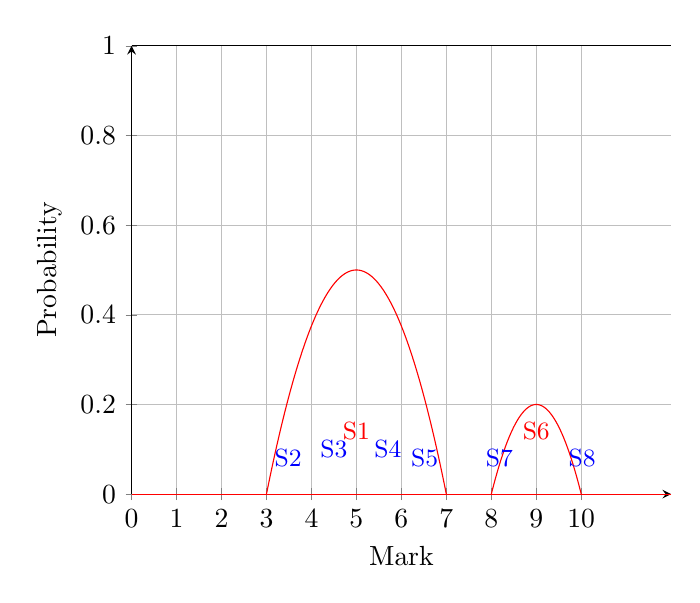
\begin{tikzpicture}
    \begin{axis}[
    		axis lines=left,
                 xtick={0,1,...,10},ytick = {0,0.2,...,1},
                 grid=both,
                 xlabel = {Mark},
                 ylabel = {Probability}
                 ]
                 %First Mode
\addplot [
    domain=3:7, 
    samples=100, 
    color=red,
]
{-0.125*x^2 + 1.25*x - 2.625};

\addplot [
    domain=0:12, 
    samples=10, 
    color=red,
    ]
    {0};
    \addplot [
    domain=0:12, 
    samples=2
  %  color=red,
    ]
    {1};
%Second mode
\addplot [
    domain=8:10, 
    samples=100, 
    color=red,
    ]
    {-0.2*x^2 + 3.6*x - 16};
 
 %First Mode

\draw[red,fill,thick] (50,50) circle (0.05cm);

 %S1
\draw[red,thick] (50,4) circle (0.2cm);
\node[red,above] at (axis cs:5,0.1){\small{S1}};
 %S2
\draw[blue,thick] (40,4) circle (0.2cm);
\node[blue,left] at (axis cs:4,0.08){\small{S2}};
 %S3
\draw[blue,thick] (45,4) circle (0.2cm);
\node[blue,above] at (axis cs:4.5,0.06){\small{S3}};
 %S4
\draw[blue,thick] (57,4) circle (0.2cm);
\node[blue,above] at (axis cs:5.7,0.06){\small{S4}};
 %S5
\draw[blue,thick] (60,4) circle (0.2cm);
\node[blue,right] at (axis cs:6,0.08){\small{S5}};

 %Second Mode
 
 \draw[red,fill,thick] (90,20) circle (0.05cm);
 %S6
\draw[red,thick] (90,4) circle (0.2cm);
\node[red,above] at (axis cs:9,0.1){\small{S6}};
 %S7
\draw[blue,thick] (87,4) circle (0.2cm);
\node[blue,left] at (axis cs:8.7,0.08){\small{S7}};
 %S8
\draw[blue,thick] (95,4) circle (0.2cm);
\node[blue,right] at (axis cs:9.5,0.08){\small{S8}};
    \end{axis}
\end{tikzpicture}


\subsection{Why?}

\subsection{How?}

\subsection{Advantages and disadvantages}

\section{Evaluation}

\begin{enumerate}[(a) ]
\item What is evaluation? Convergence(performance) | accuracy | Complexity
\item Dataset (name, source, type, image size ....)
\item Computer test configuration
\item Program language
\item Results (time | number of cluster | accuracy) ~~~> describe detail.
\item Comparison of the two methods
\end{enumerate}
	
	
\section{Conclusion}
\section{Reference}

\end{document}